\chapter{Interactive Application}\label{chap:application}

\section{Introduction}

The previous chapters presented the theoretical foundations, dataset analysis, experimental methodology, and evaluation of the Machine Learning models developed for firewall traffic classification. To make these contributions accessible through a practical interface, an interactive application was implemented using Streamlit. It provides a unified environment for exploring historical firewall records, examining their statistical characteristics, and interacting with the trained classification pipeline.

The application brings together several functionalities corresponding to the main stages of the project. It provides an overview of the dataset, tools for investigating data quality and traffic distributions, and access to statistical analyses. In addition, it integrates manual and batch prediction functionalities, allowing users to submit traffic records and obtain predicted firewall actions from the trained model. Model performance information and explanatory material are also made accessible through the interface.

Beyond providing a convenient way to interact with the classification model, the application aims to improve the interpretability and accessibility of the experimental work. By combining data exploration, statistical analysis, and model inference within a single interface, it offers a practical demonstration of how the developed Machine Learning pipeline can be used to analyze historical firewall traffic.

It is important to emphasize that the application operates on historical or user-provided traffic records. It does not intercept live network traffic, replace an existing firewall, detect intrusions, or enforce security policies. Its predictions are therefore analytical estimates based on patterns learned from the available dataset and should not be interpreted as authoritative security decisions.

This chapter presents the application's architecture and implementation, describes its main functionalities, and illustrates how users can interact with the different components. It also discusses the practical considerations and limitations associated with the resulting application.


\section{Architecture}
The application is organised around two related workflows: model preparation and model inference. The preparation workflow covers the loading and cleaning of historical firewall records, preprocessing, model training, evaluation and export of the selected pipeline. The inference workflow uses the exported pipeline within the Streamlit application to process user-provided traffic records and display the resulting predictions. Separating these workflows allows the trained model to be reused by the application without repeating the training process whenever a user requests a prediction.

The architecture also distinguishes between exploratory functions and prediction functions. The former allow users to inspect the dataset, its quality and its statistical characteristics, while the latter provide individual and batch classification. The application therefore acts as an interface to the existing analytical pipeline rather than as a live firewall or traffic-interception system.

\begin{figure}[htbp]
  \centering
  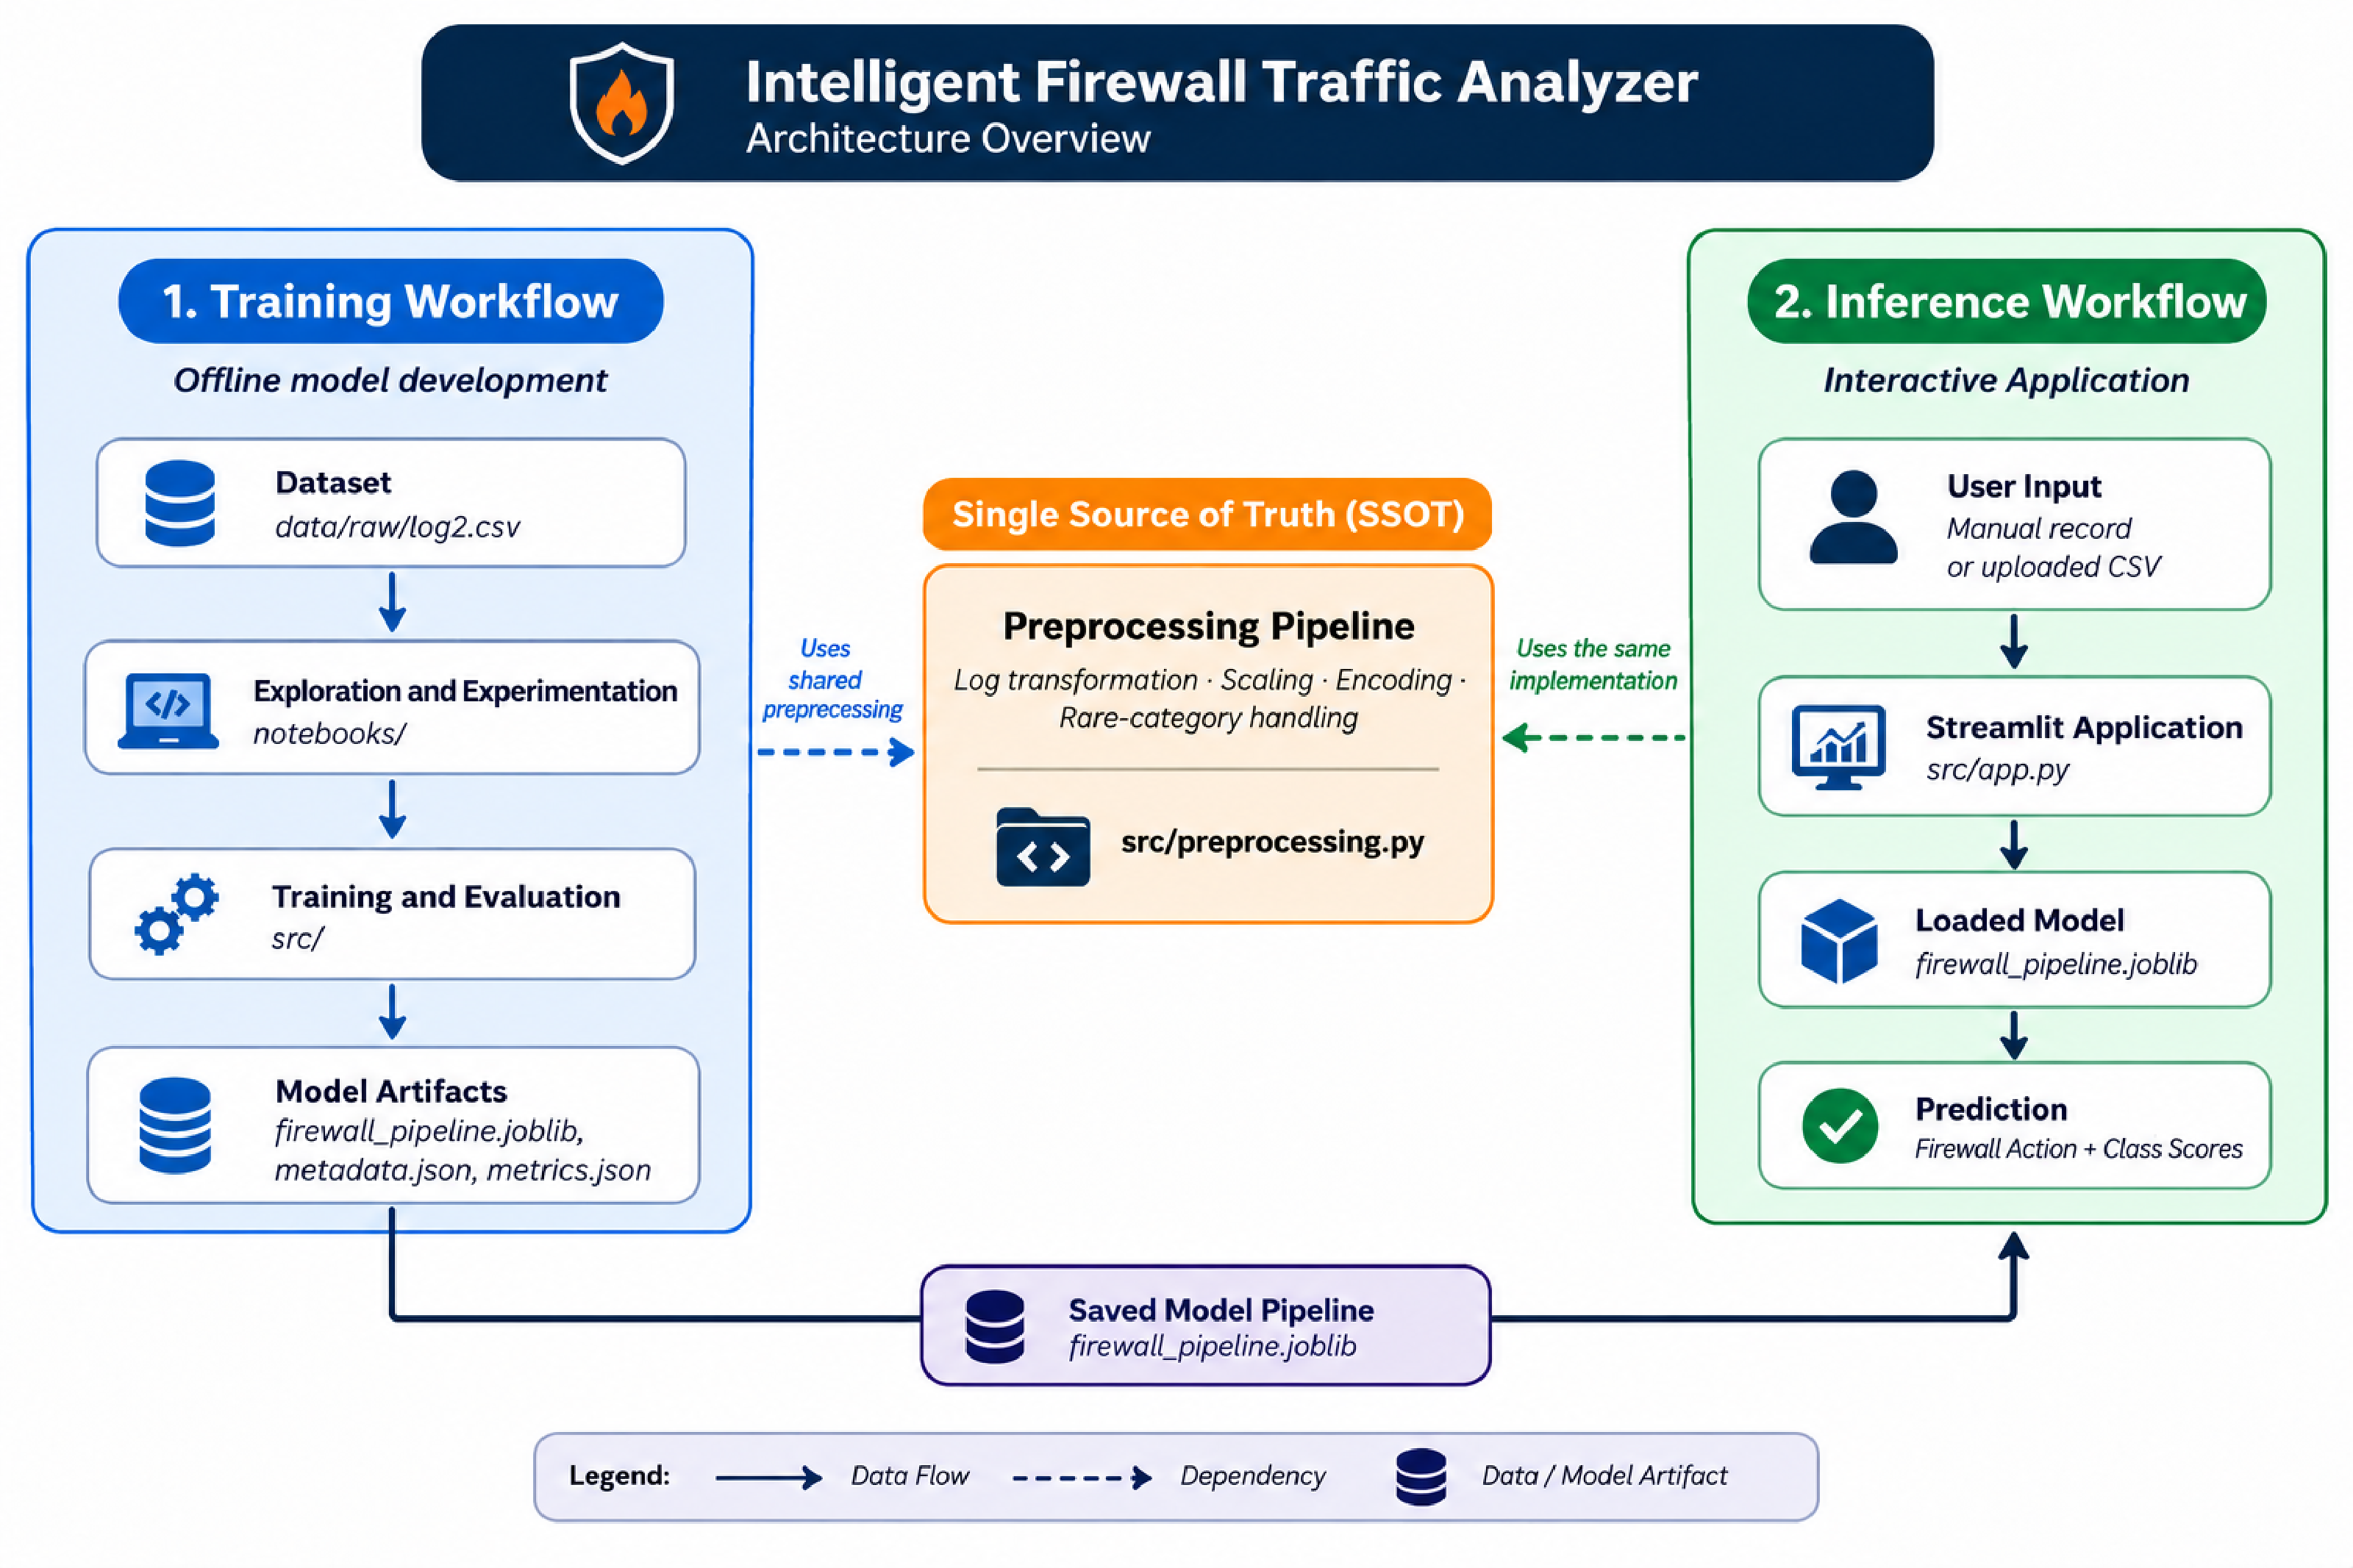
\includegraphics[width=\linewidth,height=1\textheight,keepaspectratio]{figures/ch06/Intelligent_Firewall_Architecture_Overview.pdf}
  \caption{workflows of the Intelligent Firewall Traffic Analyzer}
  \label{fig:training_inference_workflow}
\end{figure}


\section{Application Pages}
\subsection{Overview}
Summarizes the historical firewall dataset (65,532 records, 12 fields, 4 actions, 0 missing values), displays action class distribution and a raw data preview, and highlights key dataset limitations such as class imbalance and potential target leakage.
The layout and main components of this page are illustrated in	Figure~\ref{fig:overview_page}

\begin{figure}[htbp]
  \centering
  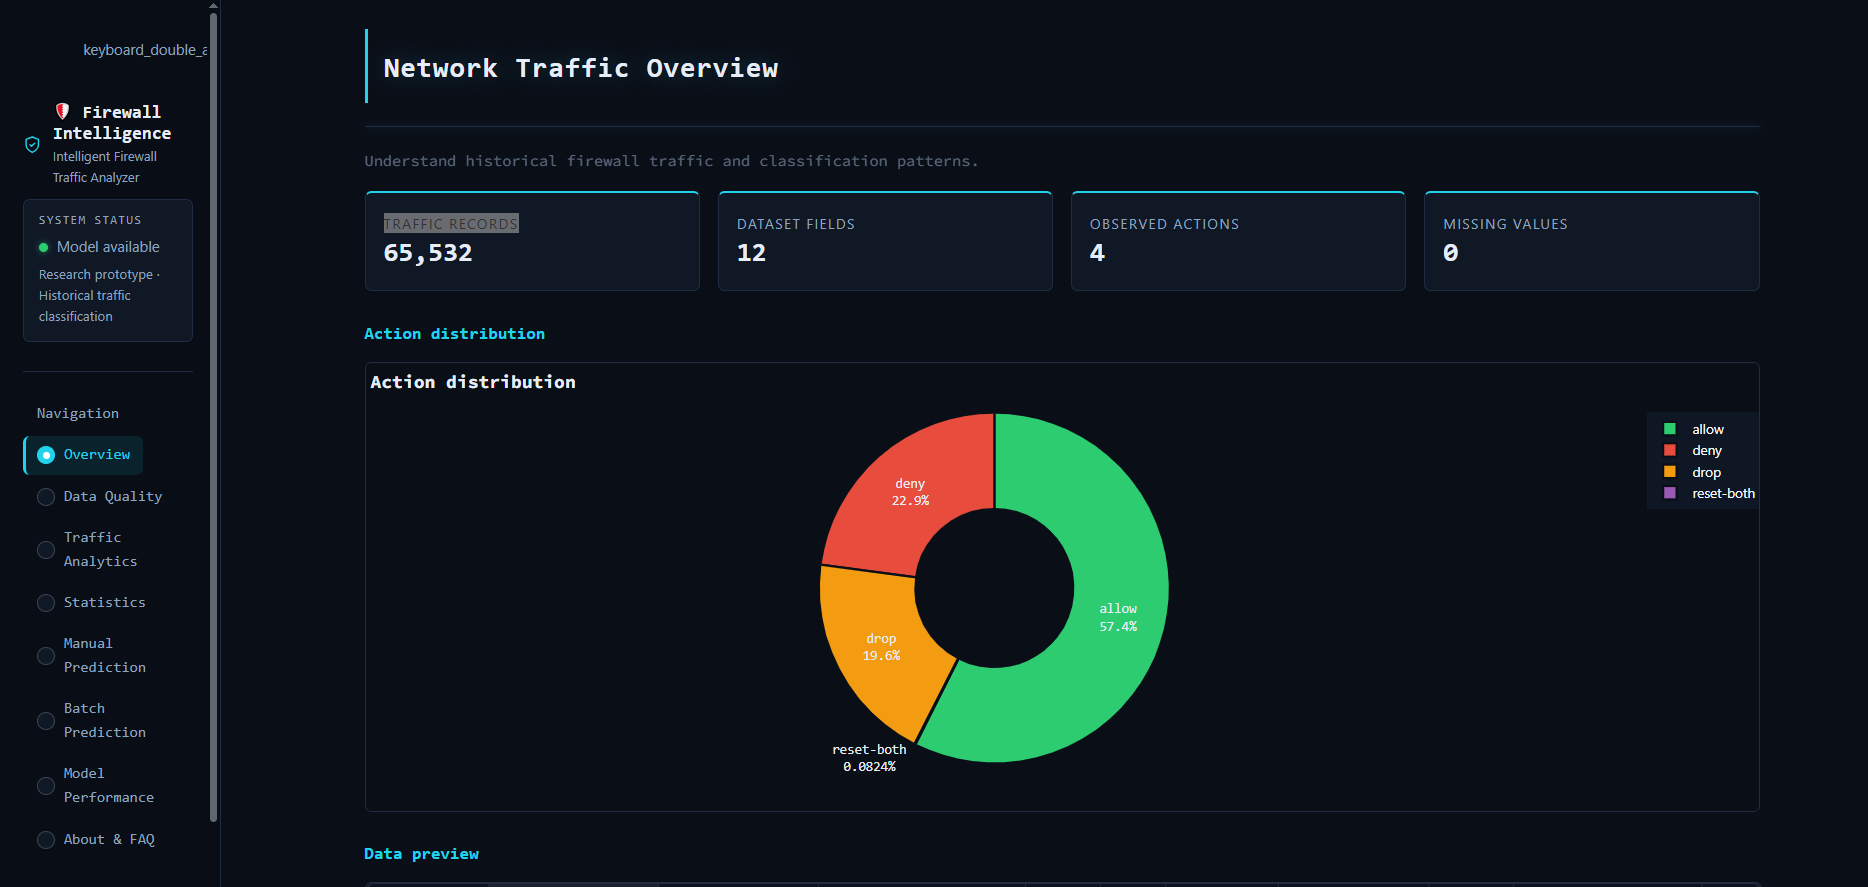
\includegraphics[width=\linewidth,height=1\textheight,keepaspectratio]{figures/ch06/1.overview page.png}
  \caption{Network Traffic Overview page}
  \label{fig:overview_page}
\end{figure}

\subsection{Data Quality}
Evaluates data quality across the full 65,532-row dataset by reporting duplicate row counts (8,362 extra copies and 57,170 distinct rows), conflicting labels across identical feature vectors (9 groups covering 46 rows), class share comparisons before and after deduplication, and outlier candidates above the 99th percentile.
The layout and main components of this page are illustrated in	Figure~\ref{fig:data_quality_page}

\begin{figure}[htbp]
  \centering
  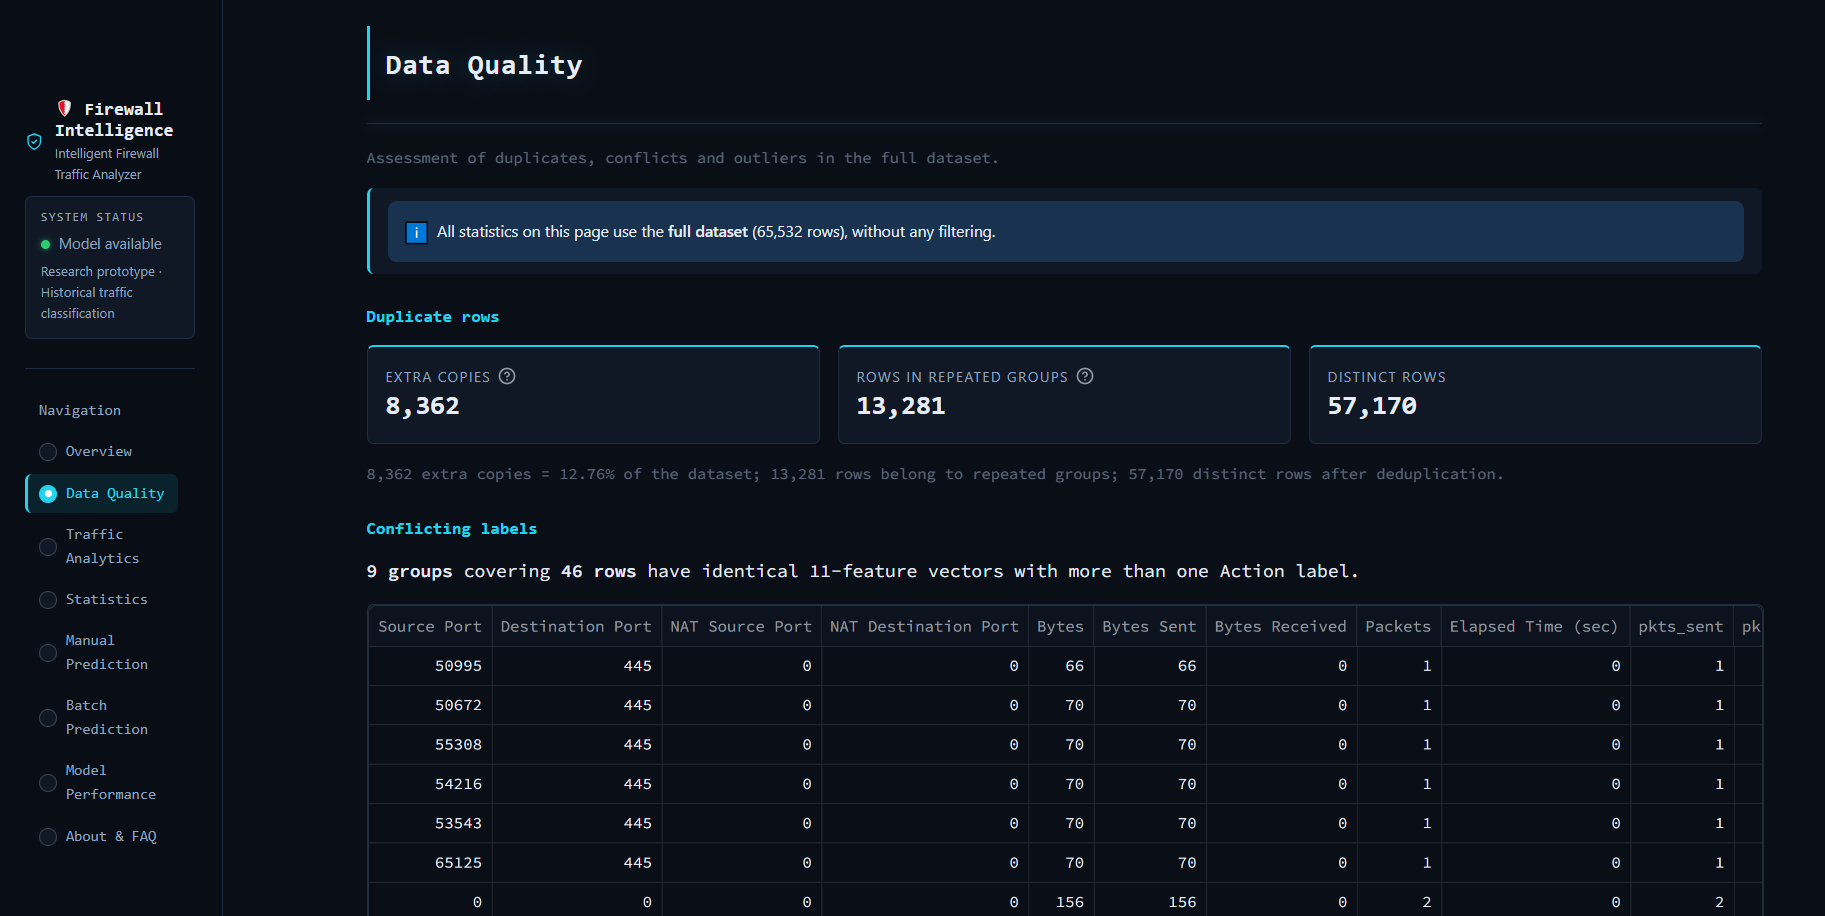
\includegraphics[width=\linewidth,height=1\textheight,keepaspectratio]{figures/ch06/2.dataqualitypage.png}
  \caption{Data Quality page}
  \label{fig:data_quality_page}
\end{figure}

\subsection{Traffic Analytics}
Provides exploratory data analysis across 65,532 selected historical firewall log records through tabs for descriptive statistics, missing values, distributions, frequencies, correlations, and a filterable data table.
The layout and main components of this page are illustrated in Figure~\ref{fig:traffic_analytics_eda_page}

\begin{figure}[htbp]
  \centering
  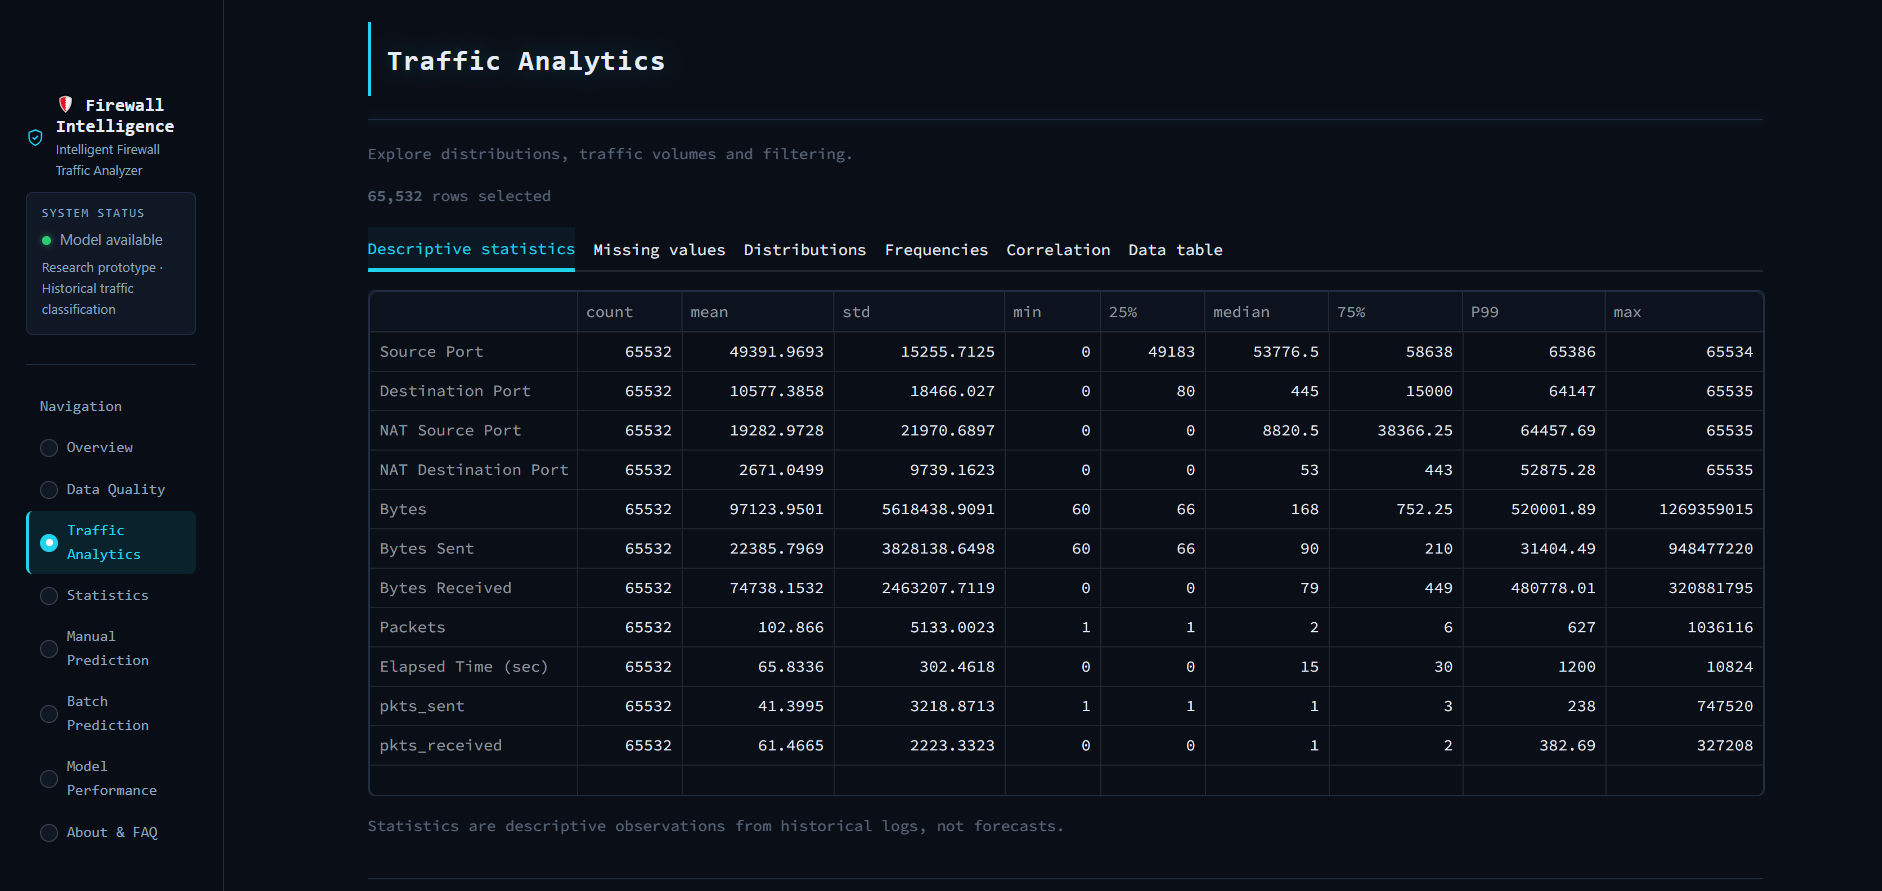
\includegraphics[width=\linewidth,height=1\textheight,keepaspectratio]{figures/ch06/3.TrafficAnalyticsEDApage.png}
  \caption{Traffic Analytics and EDA page}
  \label{fig:traffic_analytics_eda_page}
\end{figure}

\subsection{Statistics}
Presents non-parametric statistical tests comparing original and deduplicated datasets—specifically a Kruskal-Wallis H test on byte counts across action classes and a Chi-square test between NAT source port status and action—along with boxplots, heatmaps, and leakage cautions.The layout and main components of this page are illustrated in	Figure~\ref{fig:statistics_page}

\begin{figure}[htbp]
  \centering
  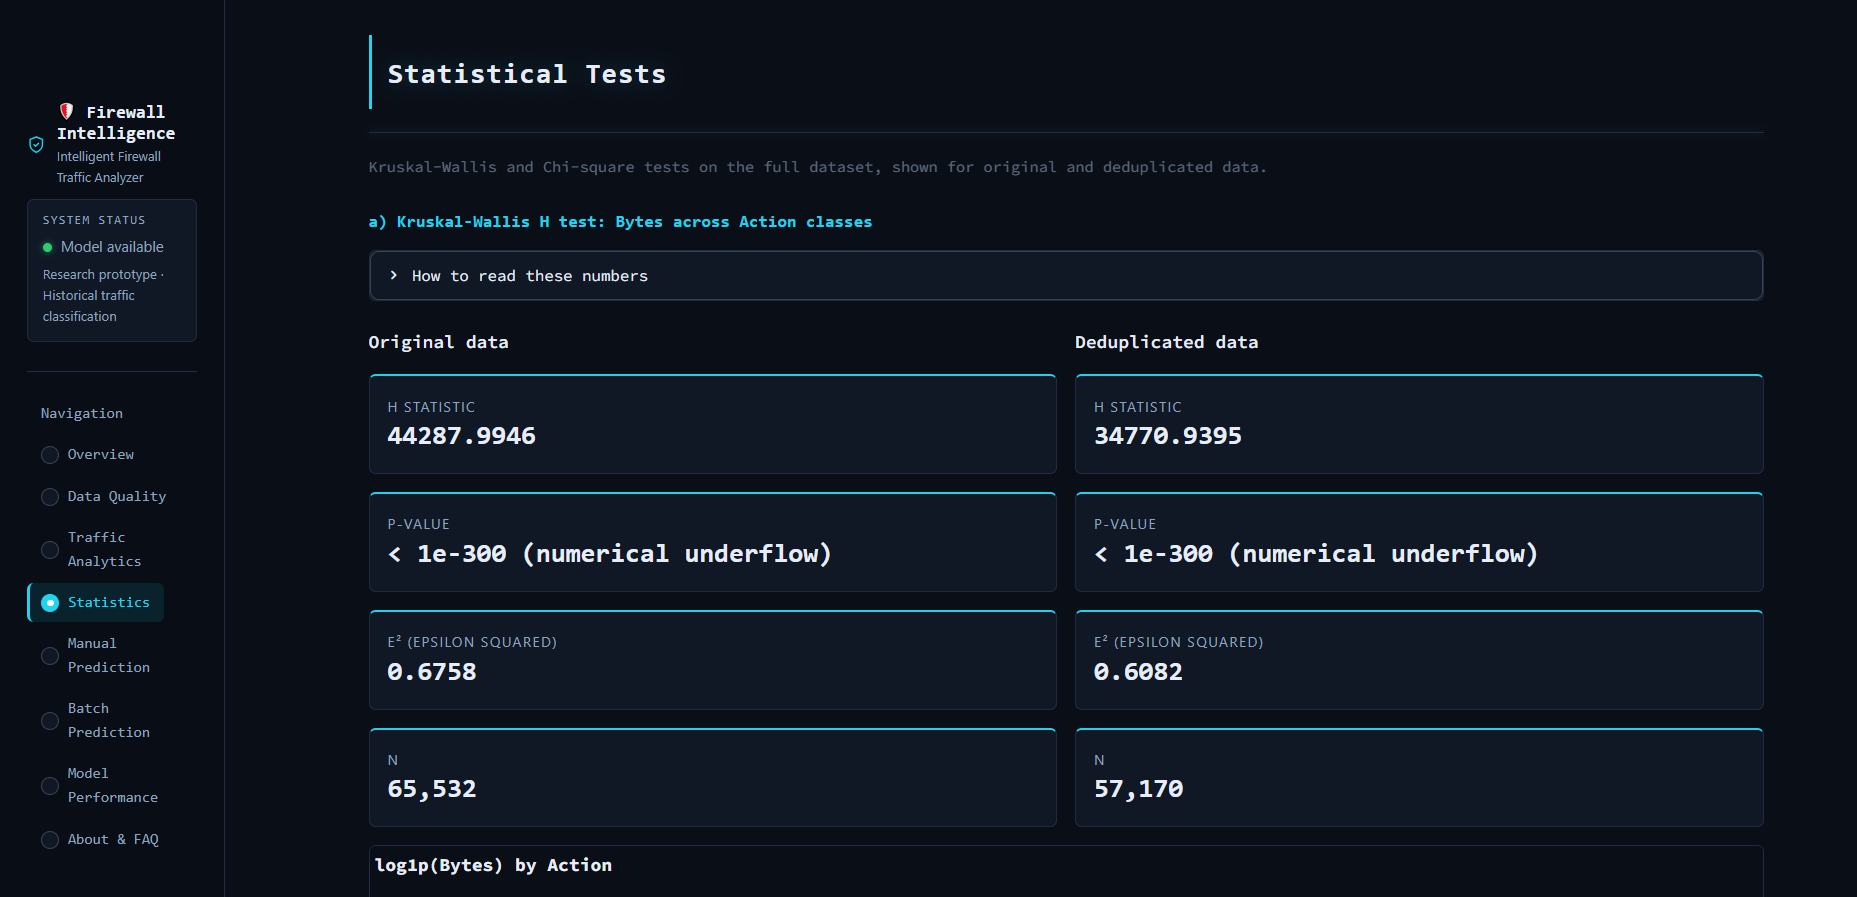
\includegraphics[width=\linewidth,height=1\textheight,keepaspectratio]{figures/ch06/4.statisticspage.png}
  \caption{Statistical Tests page}
  \label{fig:statistics_page}
\end{figure}

\subsection{Model Performance}
Displays offline evaluation results across models—including Random Forest, KNN, Decision Tree, and SVM (SVC)—covering held-out test metrics, group-aware cross-validation comparisons, feature-set ablation, a confusion matrix, per-class metrics, bar charts, and feature importances.The layout and main components of this page are illustrated in	Figure~\ref{fig:model_performance_page}

\begin{figure}[htbp]
  \centering
  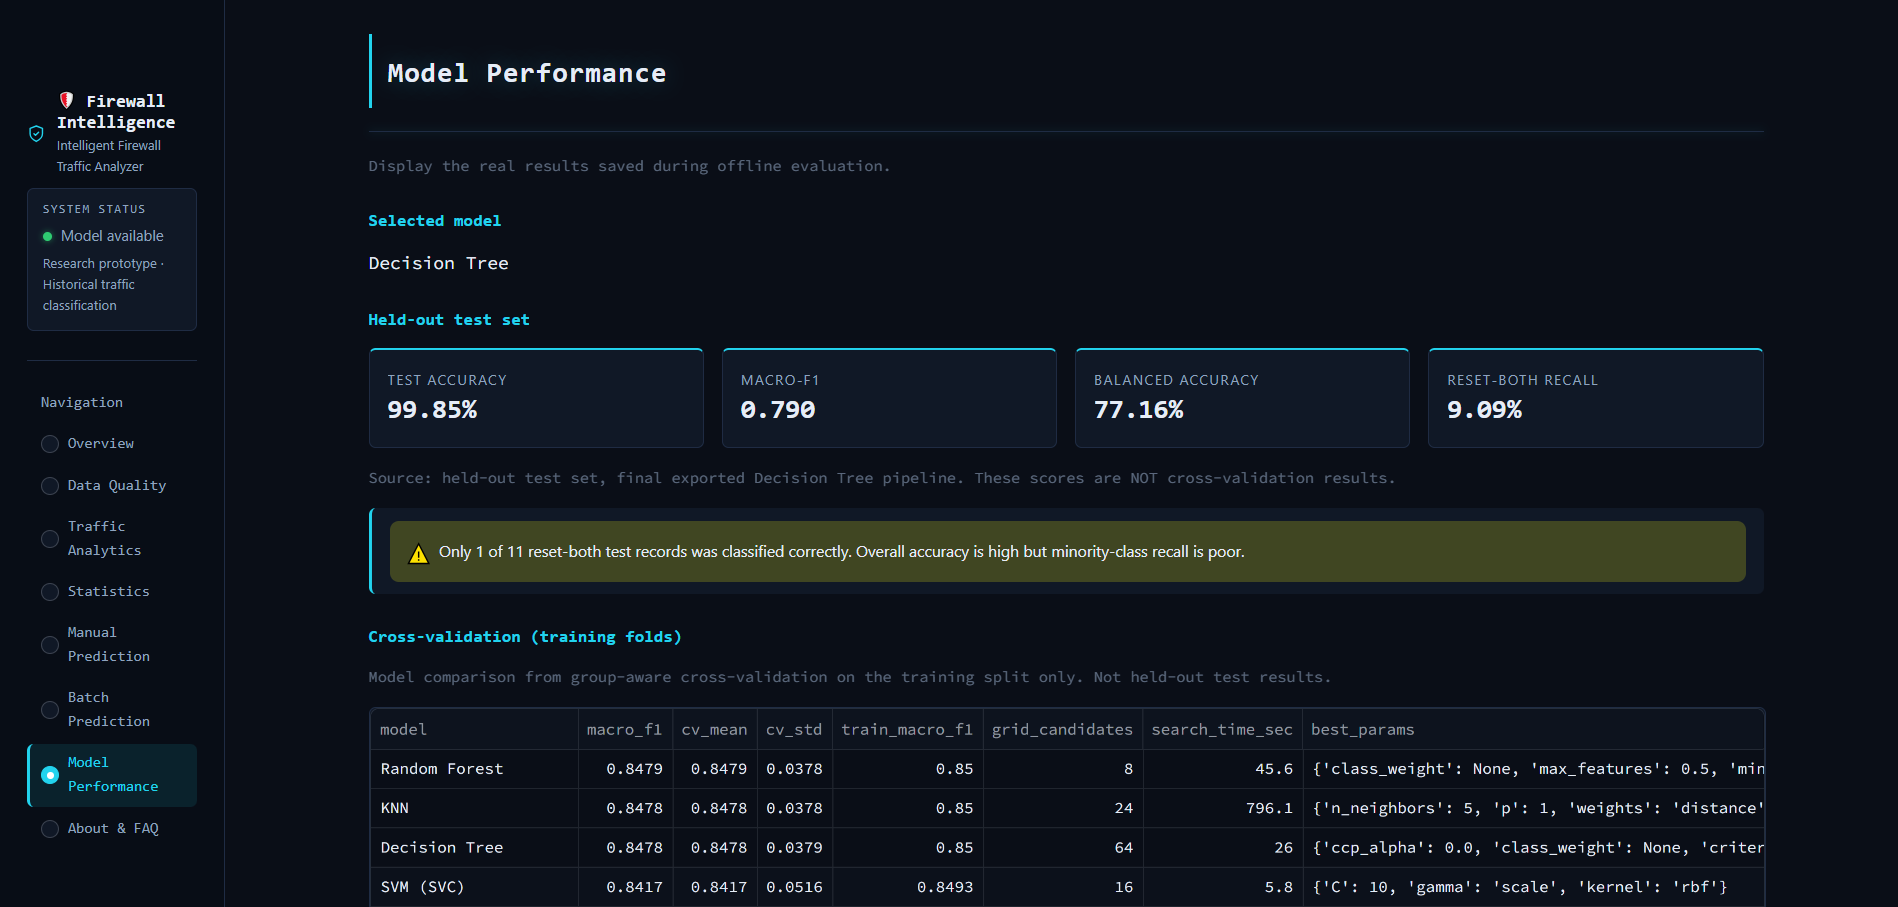
\includegraphics[width=\linewidth,height=1\textheight,keepaspectratio]{figures/ch06/5.modelperformancepage.png}
  \caption{Model Performance page}
  \label{fig:model_performance_page}
\end{figure}

\subsection{Manual Prediction}
Lets users enter or load sample network flow characteristics (such as ports, bytes, elapsed time, and packet counts) to generate a single firewall action prediction, while automatically computing total bytes and packets on submit and outlining key model limitations.
The layout and main components of this page are illustrated in	Figure~\ref{fig:manual_prediction_page}

\begin{figure}[htbp]
  \centering
  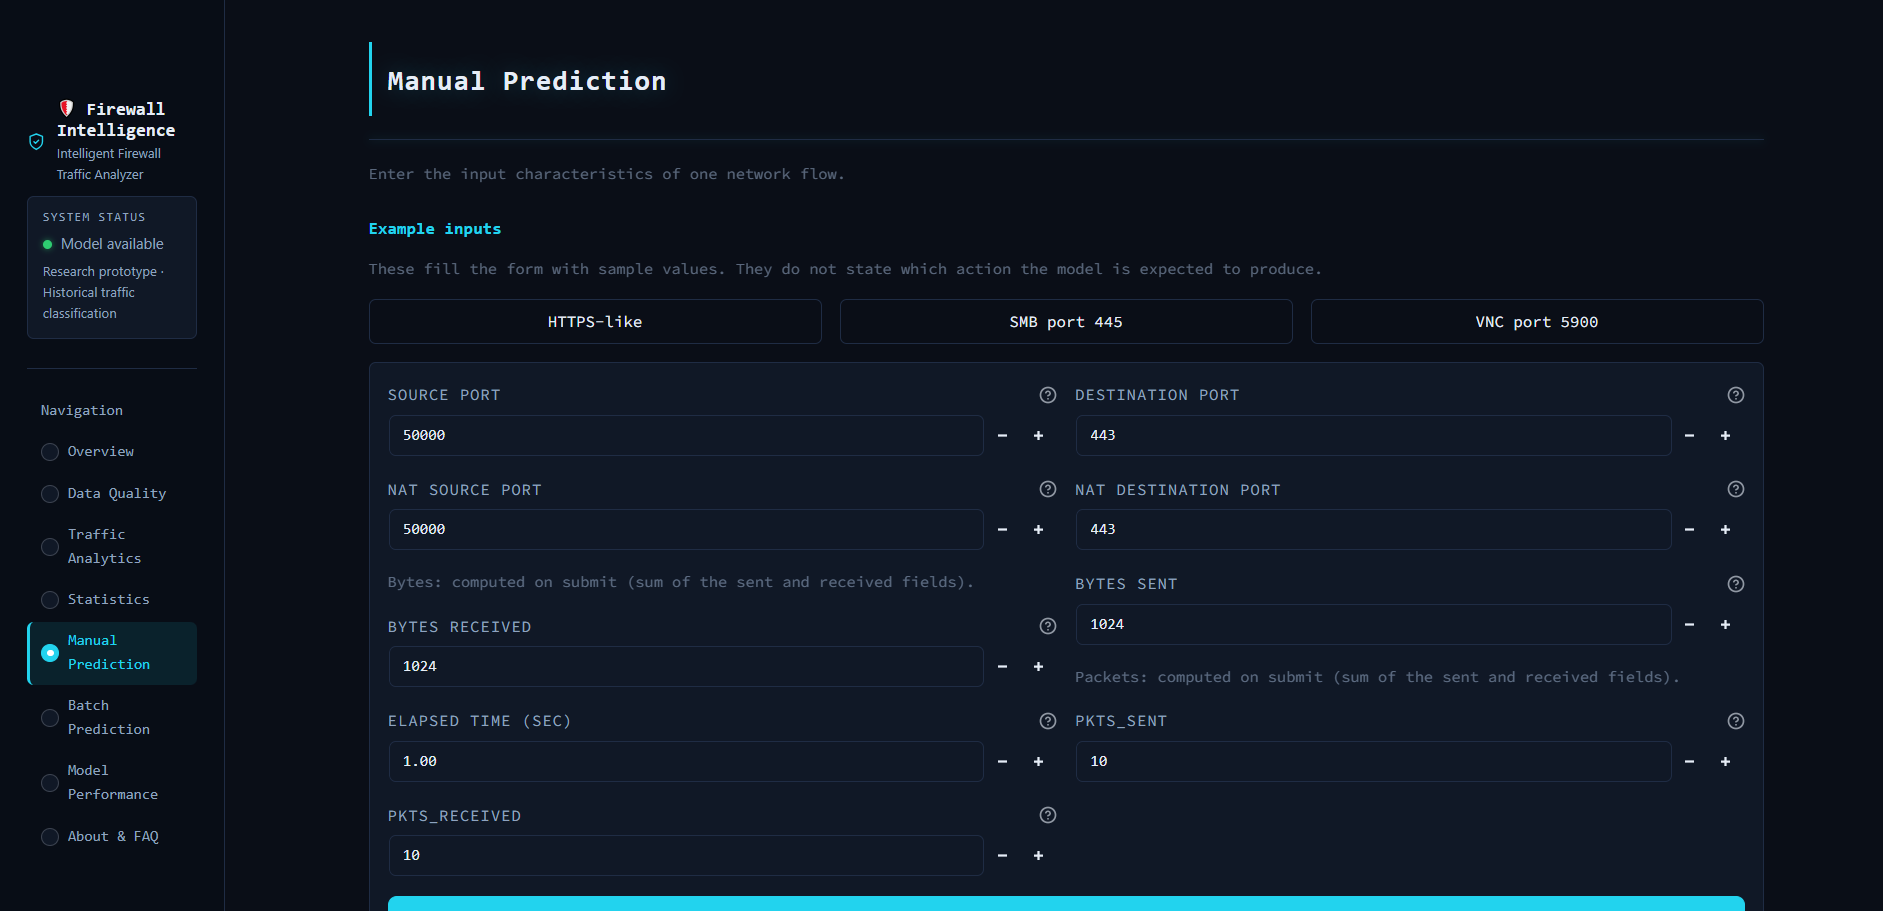
\includegraphics[width=\linewidth,height=1\textheight,keepaspectratio]{figures/ch06/6.manualpredictionpage.png}
  \caption{Manual Prediction page}
  \label{fig:manual_prediction_page}
\end{figure}

\subsection{Batch Prediction}
Allows users to download a header-only CSV template, upload a traffic CSV file (up to 20 MB) containing the required input columns, and run batch predictions to export predicted firewall actions.
The layout and main components of this page are illustrated in	Figure~\ref{fig:batch_prediction_page}

\begin{figure}[htbp]
  \centering
  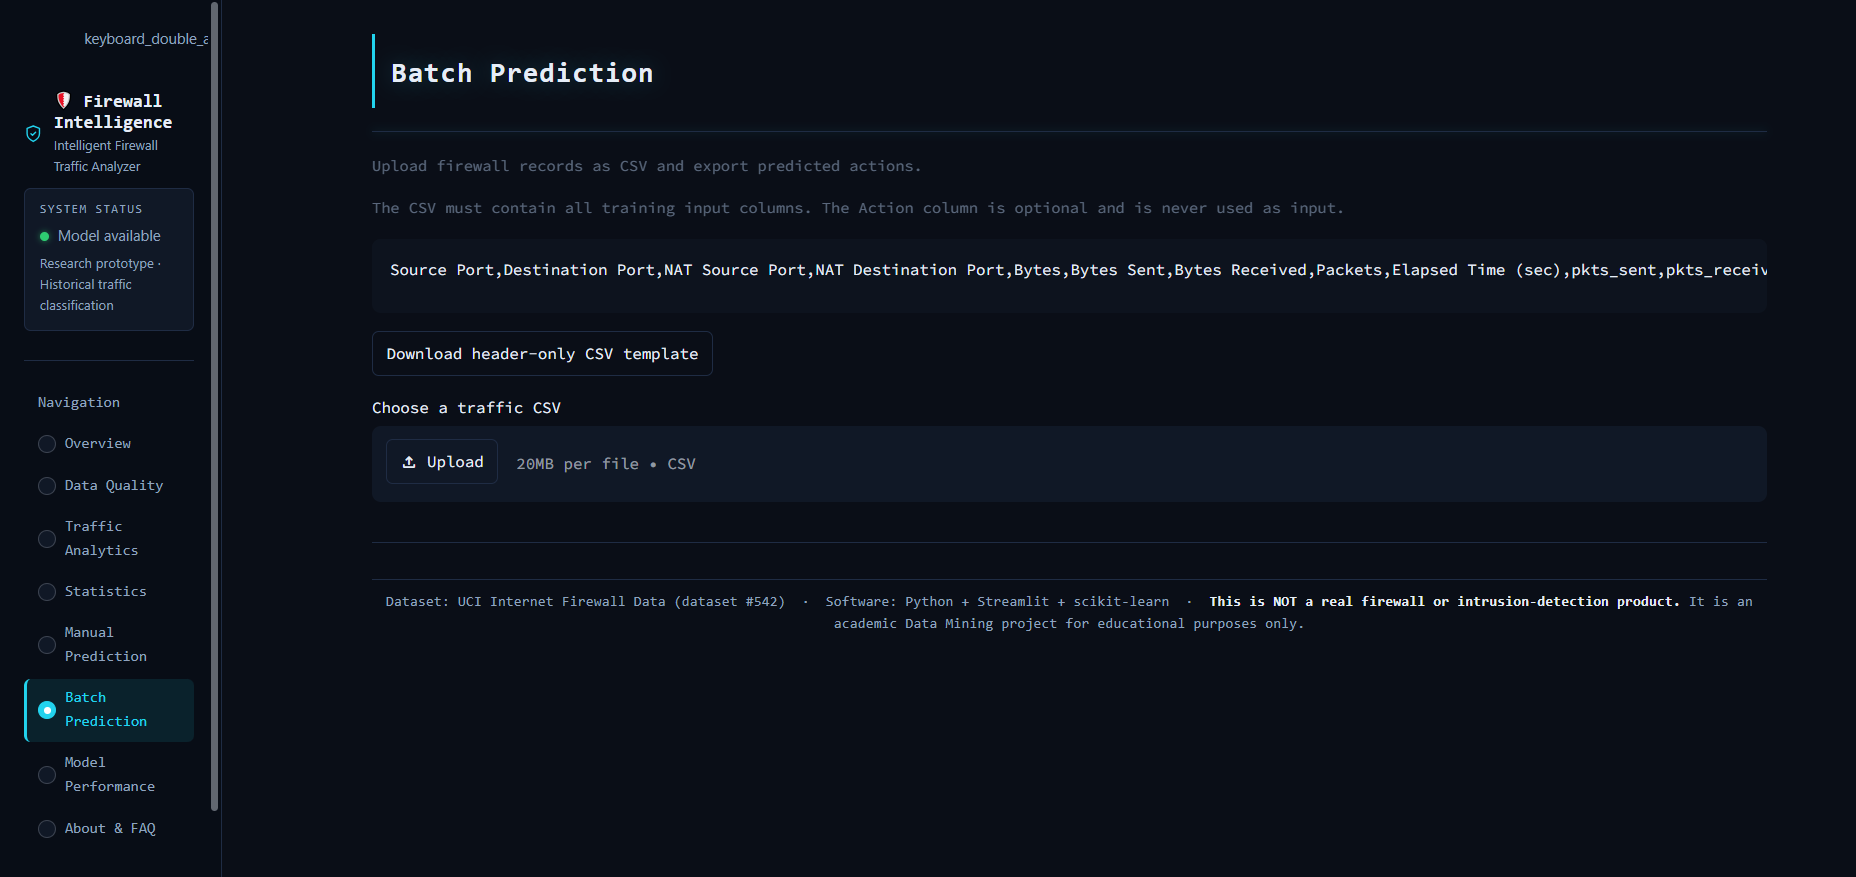
\includegraphics[width=\linewidth,height=1\textheight,keepaspectratio]{figures/ch06/7.batchpredictionpage.png}
  \caption{Batch Prediction page}
  \label{fig:batch_prediction_page}
\end{figure}



\section{Prediction Form and Input Validation}

The Manual Prediction interface allows users to manually enter network traffic characteristics and obtain a firewall action prediction using the trained Machine Learning model. It provides an interactive mechanism for testing individual network traffic records without requiring users to upload a dataset.

The interface includes nine input fields corresponding to the features used by the prediction model: Source Port, Destination Port, NAT Source Port, NAT Destination Port, Bytes Sent, Bytes Received, Packets Sent, Packets Received, and Elapsed Time (sec). Users can modify these numerical values directly through the input fields or the adjacent increment and decrement controls. The interface also provides predefined example inputs to facilitate testing with different traffic scenarios.
The layout and main components of this form are illustrated in	Figure~\ref{fig:manual_prediction_form}

\begin{figure}[htbp]
  \centering
  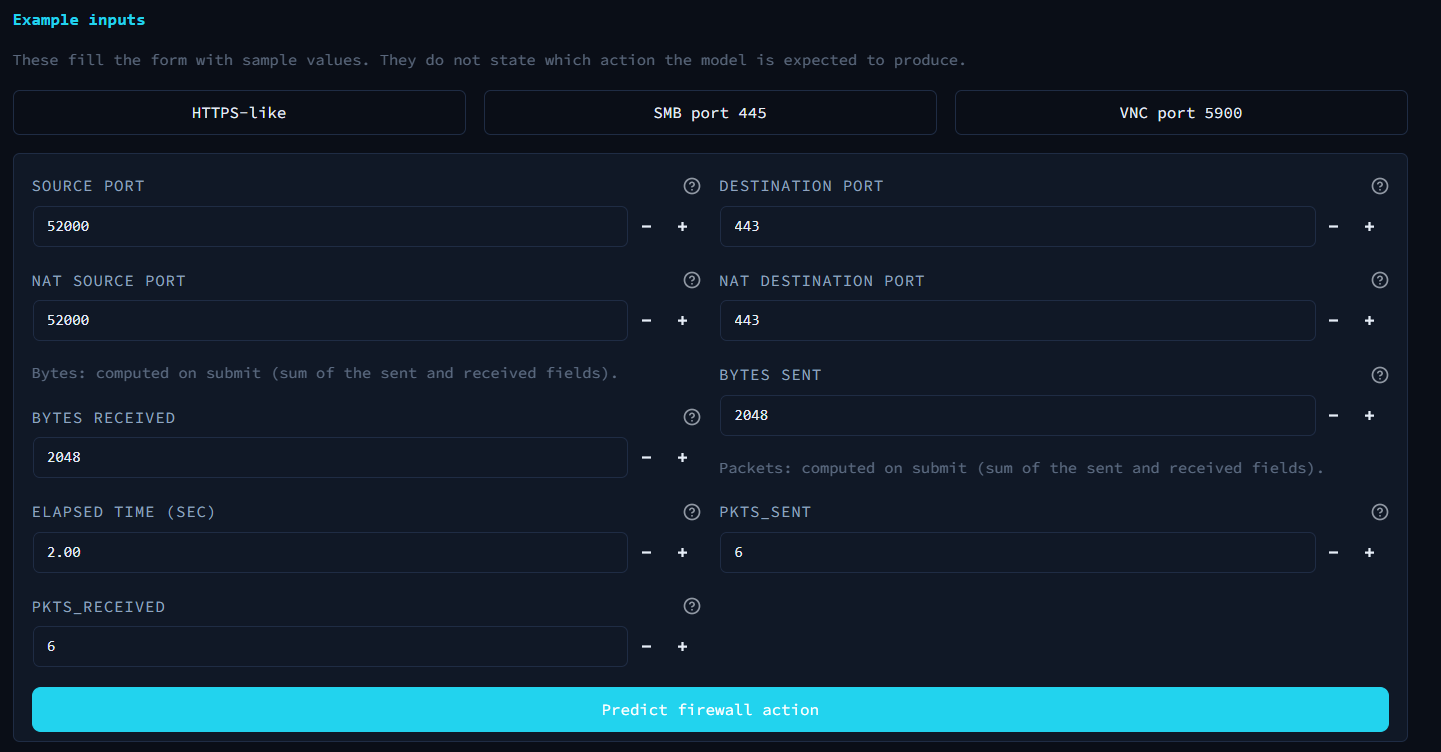
\includegraphics[width=\linewidth,height=1.5\textheight,keepaspectratio]{figures/ch06/manualpredicitionform.png}
  \caption{Manual Prediction form}
  \label{fig:manual_prediction_form}
\end{figure}



Two additional values, Total Bytes and Total Packets, are calculated automatically when the prediction is submitted. Total Bytes represents the sum of Bytes Sent and Bytes Received, while Total Packets represents the sum of Packets Sent and Packets Received.

To ensure valid input, the application applies numerical validation rules. Source and destination ports, including their NAT counterparts, must contain values between 0 and 65,535. Bytes Sent, Bytes Received, Packets Sent, Packets Received, and Elapsed Time must contain non-negative values. When an invalid value is entered, the interface visually identifies the problematic field. For example, entering a negative value such as -5 in the \texttt{PKTS\_SENT} field triggers a validation error, represented by a red border and an error indicator. This prevents invalid values from being used for prediction. illustrated in	Figure~\ref{fig:example_invalid_input}

\begin{figure}[htbp]
  \centering
  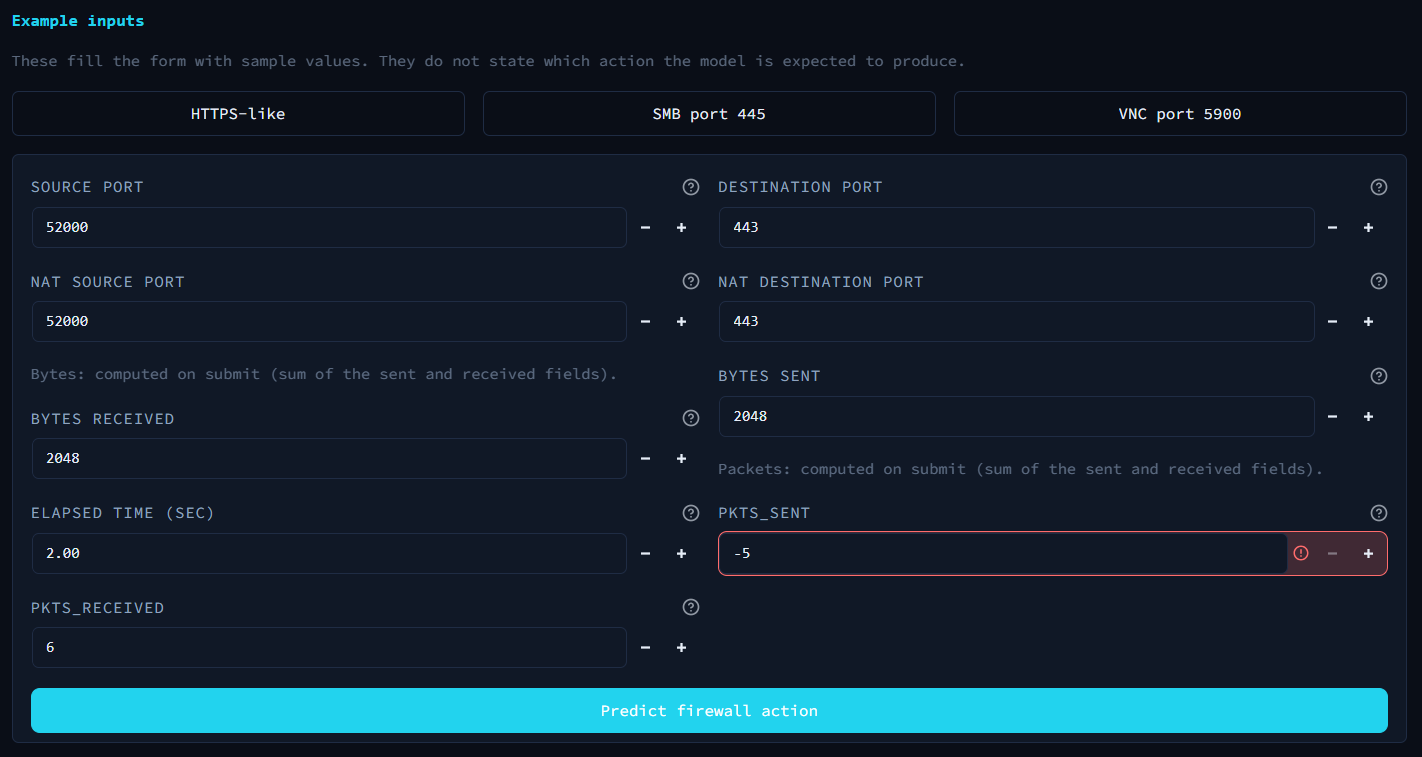
\includegraphics[width=\linewidth,height=1.5\textheight,keepaspectratio]{figures/ch06/exempleinvalidinput.png}
  \caption{Manual Prediction form showing a validation error}
  \label{fig:example_invalid_input}
\end{figure}



After entering the required characteristics, the user clicks the Predict firewall action button to execute the model. The application displays two main outputs: the predicted firewall action and the model score for each possible class. The predicted action can be one of four categories: allow, deny, drop, or reset-both. The allow action permits the network connection, deny rejects it, drop silently discards the traffic, and reset-both terminates the connection by resetting both communication endpoints.

In addition to the predicted action, the application displays a bar chart representing the model score associated with each possible firewall action. In the illustrated successful prediction, the model classified the network traffic as allow, producing a score of 100 for this class and 0 for the remaining classes (deny, drop, and reset-both). These scores represent the model's output for each class and should not automatically be interpreted as calibrated probabilities or guarantees of prediction correctness.illustrated in	Figure~\ref{fig:successful_prediction}
\begin{figure}[htbp]
  \centering
  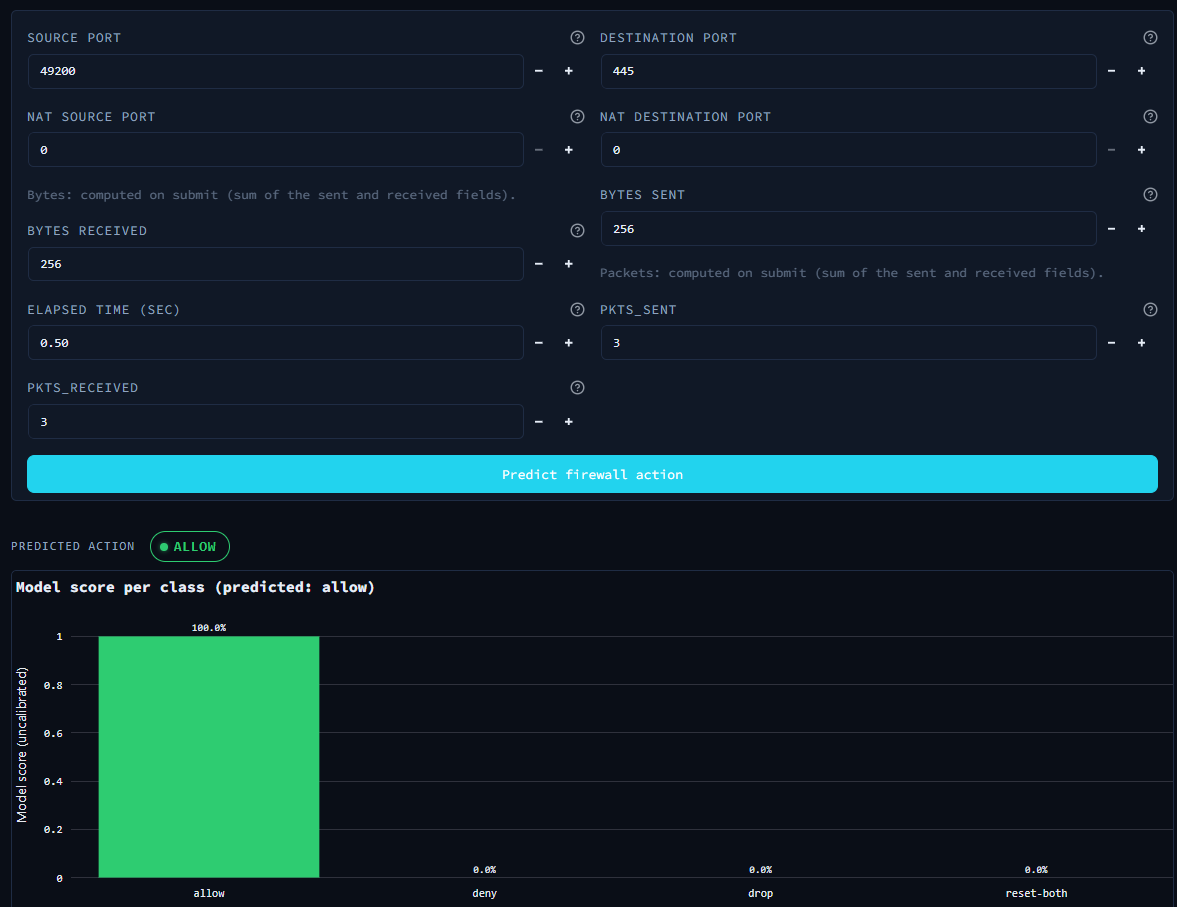
\includegraphics[width=\linewidth,height=1.5\textheight,keepaspectratio]{figures/ch06/successfulprediction.png}
  \caption{Manual Prediction output displaying prediction}
  \label{fig:successful_prediction}
\end{figure}

Although the Manual Prediction functionality provides a convenient way to evaluate individual network traffic records, its results must be interpreted within the limitations of the underlying model. First, the model was trained on historical single-policy data collected from one firewall, which may limit its ability to generalize to other firewall configurations and security policies. Second, the reset-both class contains only 43 training samples and 11 test samples after deduplication, making predictions for this class particularly uncertain.

Another important limitation concerns potential target leakage. The model may rely on NAT port patterns and byte/packet counts that reflect the firewall decision itself rather than independently predicting it. This may affect the reliability of its predictions. Finally, the generated predictions are experimental outputs intended for analysis and demonstration purposes. They must not be considered actual security policies or used directly to enforce firewall rules.

In conclusion, the Manual Prediction interface provides an interactive mechanism for entering network traffic characteristics, validating user inputs, and observing the classification results produced by the trained model. Nevertheless, its predictions should be considered experimental decision-support outputs rather than authoritative firewall security decisions.

\section{Conclusion}
In summary, this chapter presented the design, implementation, and usage of the Streamlit-based interactive application for firewall traffic classification. By bringing together dataset overview, data quality checks, exploratory analytics, non-parametric statistical tests, offline model evaluation, and both single-record and batch prediction workflows, the interface turns the underlying Machine Learning pipeline into an accessible tool for inspecting historical network traffic. At the same time, input validation, transparent evaluation metrics, and explicit warnings regarding class imbalance, single-policy scope, potential target leakage, and non-operational use keep results grounded as analytical insights rather than live security enforcement.